\documentclass[11pt,a4paper]{article}

\usepackage{titling}
\usepackage[hidelinks]{hyperref}
\usepackage{graphicx}
\usepackage{grffile}
\usepackage{float}
\usepackage{geometry}
\usepackage{listings}
\lstset{
	frame=single,
	breaklines=true,
}

\newcommand{\subtitle}[1]{
  \posttitle{
    \par\end{center}
    \begin{center}\large#1\end{center}
    \vskip0.5em}
}

\begin{document}


\title{HyperPerform\\ User Manual}
\subtitle{ Organisation: \url{https://github.com/HyperPerform}}
\begin{figure}
			\centering
			
\includegraphics[height=200px]{../Images/CodusMaximus_logo.jpg}
\end{figure}

	
\author{
	\textbf{Developers:} \\
	Rohan Chhipa		\emph{14188377}	\\
	Claudio Da Silva	\emph{14205892}	\\
	Jason Gordon		\emph{14405025}	\\
	Avinash Singh		\emph{14043778}	\\\\
}

\date{\textbf{Updated \today}}

\maketitle
\thispagestyle{empty}
\pagebreak

\tableofcontents
\pagebreak

\section{System Overview}
Many different tools are available for measuring the quality of products made, but very few tools exist which assess the quality of the people making said products. People play a huge role in a project, and trying to monitor each and every one becomes a tedious task which diverts man power away from other more critical tasks. Whether it be for an end of year evaluation, or attempting to assess the current status of a project, generating a report on a staff member can help keep up productivity, as well as get them any help they need in order to resume quality performance. By ensuring that there is constant quality performance from each individual on a project, one can increase project quality as well as reduce project risks such as loss of an important team member during a critical stage of a project's life-cycle. 

\section{System Configuration}
This guide has been made for users using a Linux based operating system. To install the HyperPerform system on the machine you will be required to have an active connection to the internet. Please note that high amounts of data might be consumed. 

\subsection{Docker installation}
To install system with ease and avoid all configurations you can download Docker. Docker can be found at \url{www.docker.com} where guides are made available for installing docker on a particular operating system. If you intend to use Docker to install the HyperPerform system then please ensure you install Docker on your machine.

\subsection{Manual Installation}
The manual installation requires you to download the source code from the GitHub repository. The newest release is highly recommended. To carry out a manual installation please ensure you have Maven and the WildFly application server on your machine. \\ \\
Maven can be downloaded from: \url{maven.apache.org} \\ \\
WildFly can be downloaded from: \url{wildfly.org} \\ \\
Please ensure you download WildFly 10. The HyperPerform system was fully tested on this version of WildFly. Any other version might produce unexpected behaviour. \\ \\
For the front-end Dashboard please ensure you have Nodejs (version 6.4.0 or higher) installed on your machine. Nodejs can be found at \url{https://nodejs.org/en/}.

\section{Installation}

\subsection{Docker Installation}

Assuming you have docker installed on your machine, simply run the following command in terminal: 

\begin{lstlisting}[language=bash]
docker run hyperperform/HyperPerform 
\end{lstlisting}
This will download the HyperPerform Docker image from DockerHub and run it on you machine. \\ \\
The front end component does not have a Docker image at this point in time. To install the front end component please look at section 3.2.5 for the manual installation.

\subsection{Manual Installation}
This installation guide assumes a Linux Server running Ubuntu 14 or higher:

\subsubsection{WildFly}
Once you have downloaded the WildFly application server please carry out the WildFly installations and add a user. Once this is done proceed to installing PostgreSQL.

%Elevate to sudo permissions:

%\begin{lstlisting}
%sudo -s
%\end{lstlisting}
%Install Java JDK 8:
%\begin{lstlisting}
%aptitude update
%aptitude install --with-recommends software-properties-common
%add-apt-repository ppa:webupd8team/java
%aptitude update
%aptitude --with-recommends install oracle-java8-installer vim
%\end{lstlisting}
%Create a WildFly user:
%\begin{lstlisting}
%adduser --no-create-home --disabled-password --disabled-login wildfly
%\end{lstlisting}
%Download and extract the WildFly installation:
%\begin{lstlisting}
%cd /opt
%wget --tries=0 --continue http://download.jboss.org/wildfly/10.0.0.Final/wildfly-10.0.0.Final.tar.gz
%tar -xzvf wildfly-10.0.0.Final.tar.gz
%ln -s wildfly-10.0.0.Final wildfly
%chown -R wildfly wildfly
%\end{lstlisting}
%\pagebreak
%Copy the initialization scripts to the required folders:
%\begin{lstlisting}
%cp /opt/wildfly/docs/contrib/scripts/init.d/wildfly-init-debian.sh /etc/init.d/wildfly
%update-rc.d /etc/init.d/wildfly defaults
%cp /opt/wildfly/docs/contrib/scripts/init.d/wildfly.conf /etc/default/wildfly
%cd /etc/default
%\end{lstlisting}
%Now to edit the files:
%\begin{lstlisting}
%nano wildfly
%\end{lstlisting}
%Uncomment and/or Edit the following lines:
%\begin{lstlisting}
%JBOSS_HOME="/opt/wildfly"
%JBOSS_USER=wildfly
%JBOSS_MODE=standalone
%JBOSS_CONFIG=standalone-full.xml
%JBOSS_CONSOLE_LOG="/var/log/wildfly/console.log"
%\end{lstlisting}
%Change all 127.0.0.1 in standalone-full.xml to 0.0.0.0, then run the following commands:
%\begin{lstlisting}
%service wildfly start
%cd /opt/wildfly/bin
%./add-user.sh
%\end{lstlisting}

\subsubsection{PostgreSQL}
The install PostgreSQL on your machine: \\\\
Install via terminal:
\begin{lstlisting}
sudo apt-get update
sudo apt-get install postgresql postgresql-contrib
\end{lstlisting}
To configure PostgreSQL to connect remotely:
\begin{lstlisting}
sudo nano /etc/postgresql/9.3/main/postgresql.conf
\end{lstlisting}
Edit the following lines:
\begin{lstlisting}
listen_addresses = "*"
\end{lstlisting}
\pagebreak


\textbf{Create database hyperperform and the tables}\\
Run the following commands in terminal: 
\begin{lstlisting}
   psql -c 'CREATE DATABASE hyperperform;' -U postgres
  
   psql -d hyperperform -c 'CREATE TABLE public."GitPush" ( id integer NOT NULL, repository character varying(255), "timestamp" timestamp without time zone, username character varying(255), commitsize integer, CONSTRAINT "GitPush_pkey" PRIMARY KEY (id) ); CREATE SEQUENCE public.hibernate_sequence INCREMENT 1 MINVALUE 1 MAXVALUE 9223372036854775807 START 1 CACHE 1;' -U postgres
  
   psql -d hyperperform -c 'CREATE TABLE public."TravisEvent" ( id integer NOT NULL, branch character varying(255), commiter character varying(255), repo character varying(255), status character varying(255), "timestamp" timestamp without time zone, CONSTRAINT "TravisEvent_pkey" PRIMARY KEY (id));' -U postgres
  
   psql -d hyperperform -c 'CREATE TABLE public."CalendarProject" ( projectid integer NOT NULL, calendarid character varying(255), collaborators bytea, creator character varying(255), duedate timestamp without time zone, eventid character varying(255), reponame character varying(255), "timestamp" timestamp without time zone, CONSTRAINT "CalendarProject_pkey" PRIMARY KEY (projectid));' -U postgres
  
   psql -d hyperperform -c 'CREATE TABLE public."CalendarMeeting" ( meetingid integer NOT NULL, calendarid character varying(255), creator character varying(255), duedate timestamp without time zone, eventid character varying(255), location character varying(255), "timestamp" timestamp without time zone, CONSTRAINT "CalendarMeeting_pkey" PRIMARY KEY (meetingid));' -U postgres
  
   psql -d hyperperform -c 'CREATE TABLE public."CalendarMeeting_attendees" ( "CalendarMeeting_meetingID" integer NOT NULL, attendees integer, attendees_key character varying(255) NOT NULL, CONSTRAINT "CalendarMeeting_attendees_pkey" PRIMARY KEY ("CalendarMeeting_meetingID", attendees_key), CONSTRAINT fkn4q1pmj9vx3tfsaw9irp9voax FOREIGN KEY ("CalendarMeeting_meetingID") REFERENCES public."CalendarMeeting" (meetingid) MATCH SIMPLE ON UPDATE NO ACTION ON DELETE NO ACTION);' -U postgres
  
   psql -d hyperperform -c 'CREATE TABLE public."GitIssue"(id integer NOT NULL, action character varying(255), assignee character varying(255), createdby character varying(255), issueid bigint, repository character varying(255), "timestamp" timestamp without time zone, CONSTRAINT "GitIssue_pkey" PRIMARY KEY (id));' -U postgres

\end{lstlisting}


\subsubsection{ActiveMQ}
To setup ActiveMQ on your server: \\
\begin{itemize}
	\item Start up your WildFly application server
	\item Navigate to WildFly management console on localhost:9990
	\item Navigate to configurations tab and click on sub-systems
	\item Scroll down and search for Messaging-ActiveMQ and click on it
	\item Click on default, select queues/topics
	\item Click add and input the following information:
		\begin{itemize}
			\item Name*: hyperperform
			\item JNDI Names*: java:/jms/queue/hyperperform
		\end{itemize}
	\item Click save \\
\end{itemize}

\subsubsection{Deploying to WildFly}
To deploy the HyperPerform system to the application you will need to build the system using from the source code. 

\begin{itemize}
	\item Ensure the WildFly server is running.
	\item Navigate to \url{https://github.com/HyperPerform/hyper-perform-server/releases} and download the newest release source code.
	\item Extract the source code
	\item Navigate to the root directory of the source code. A file named pom.xml should be clearly visible.
	\item Run the following command: mvn clean wildfly:deploy
	\item Maven will then ask you to provide your user name and password for the Wildfly Server.
	\item Thereafter Maven will automatically deploy the compiled code (war) to WildFly
\end{itemize}



\subsubsection{Front-end Dashboard}
Please notee that there is no release yet for the dashboard and there might be a few bugs, or limitations to the software.\\
To start up the front end please ensure you have Node 6.4.0 or higher installed on your machine. Node can be found at \url{https://nodejs.org/en/}. \\\\\\
\noindent
\textbf{Please make sure that these commands execute successfully before attempting to run the system:}
\begin{lstlisting}
	 npm install -g gulp
	 npm install -g bower
	 npm install -g sass
\end{lstlisting}
Once that has completed with no errors do the following.
\begin{itemize}
	\item Download the Dashboard source code from \url{https://github.com/HyperPerform/hyper-perform-web-application}
	\item Navigate to the root directory of the source code
\end{itemize}
Run the following commands in terminal: 
\begin{lstlisting}	
	npm install
	gulp build
	gulp serve
\end{lstlisting}
\noindent
The front-end system will auto launch in your default browser in order to view the data in the front-end system the Wildfly application server must be running.

%\pagebreak

%\section{Installation of HyperPerform}
%
%\subsection{Server}
%To setup the back end, take the hyperperform.war and deploy it on the WildFly management console
%
%\subsection{Dashboard}
%To install the dashboard on your server:
%\begin{lstlisting}
%npm install hyperperform
%\end{lstlisting}

\section{Getting Started/Using the System}
Once the front-end Dashboard is served your default browser should automatically open. In the event that it didn't, simply open the browser of your choice and navigate to the following URL: \url{localhost:3000}. \\ \\
Once the Dashboard loads you will be presented with the following screen:

\begin{figure}[H]
	\begin{center}
		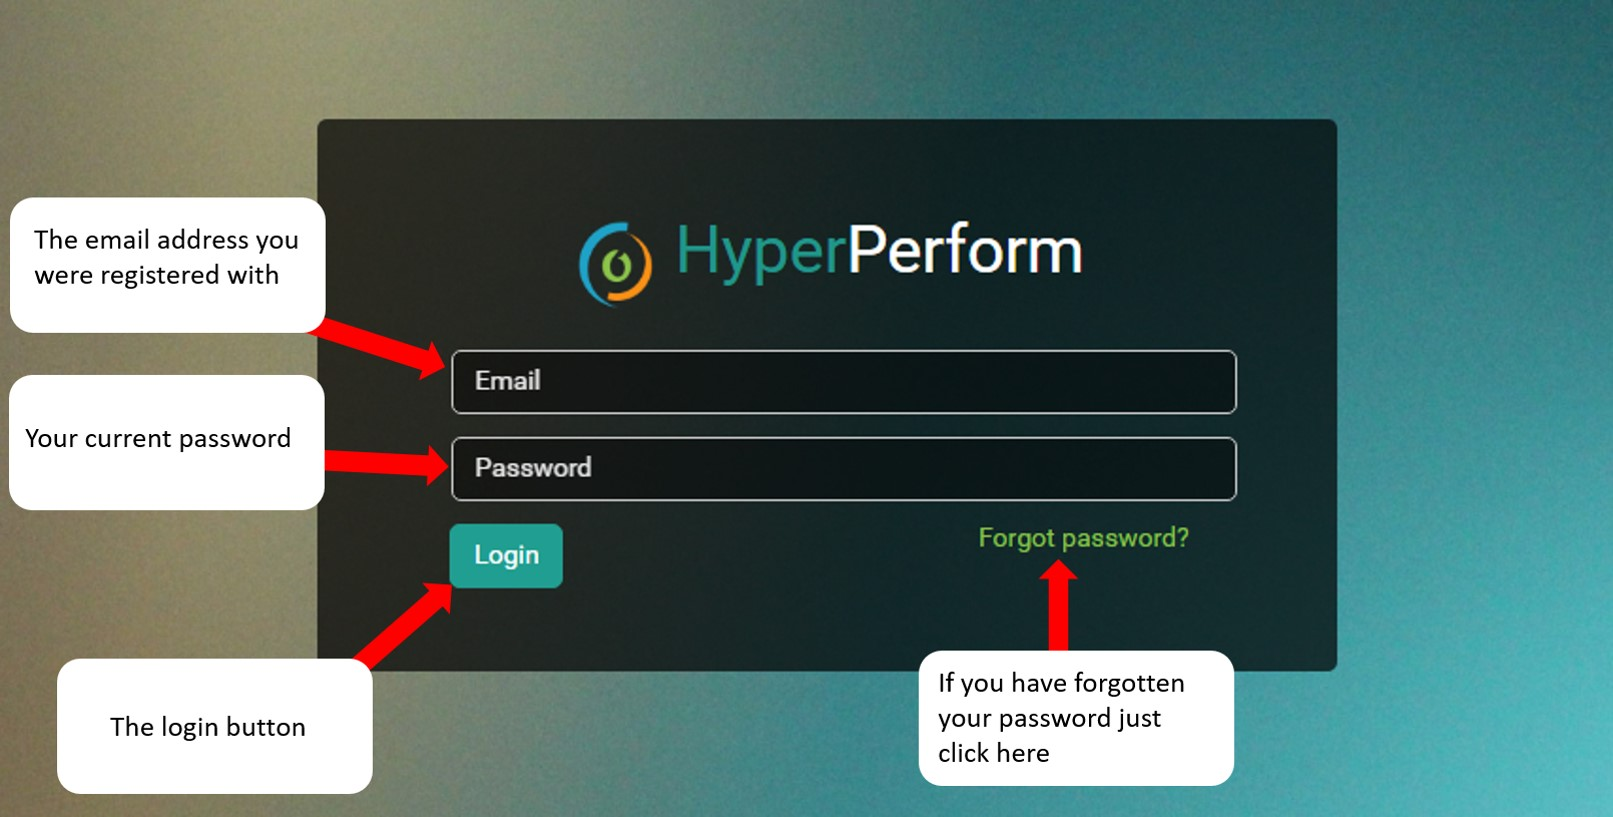
\includegraphics[scale=0.3]{../Images/Login_Screen.jpg}
		\caption{Login screen}
	\end{center}
\end{figure}
\noindent
The default username and password is Admin. This is a default login for when the system is installed for the first time. Once managers exist within the database this feature will be disabled for security purposes. \\ \\
Once logged in the user will be presented with the following screen:

\begin{figure}[H]
	\begin{center}
		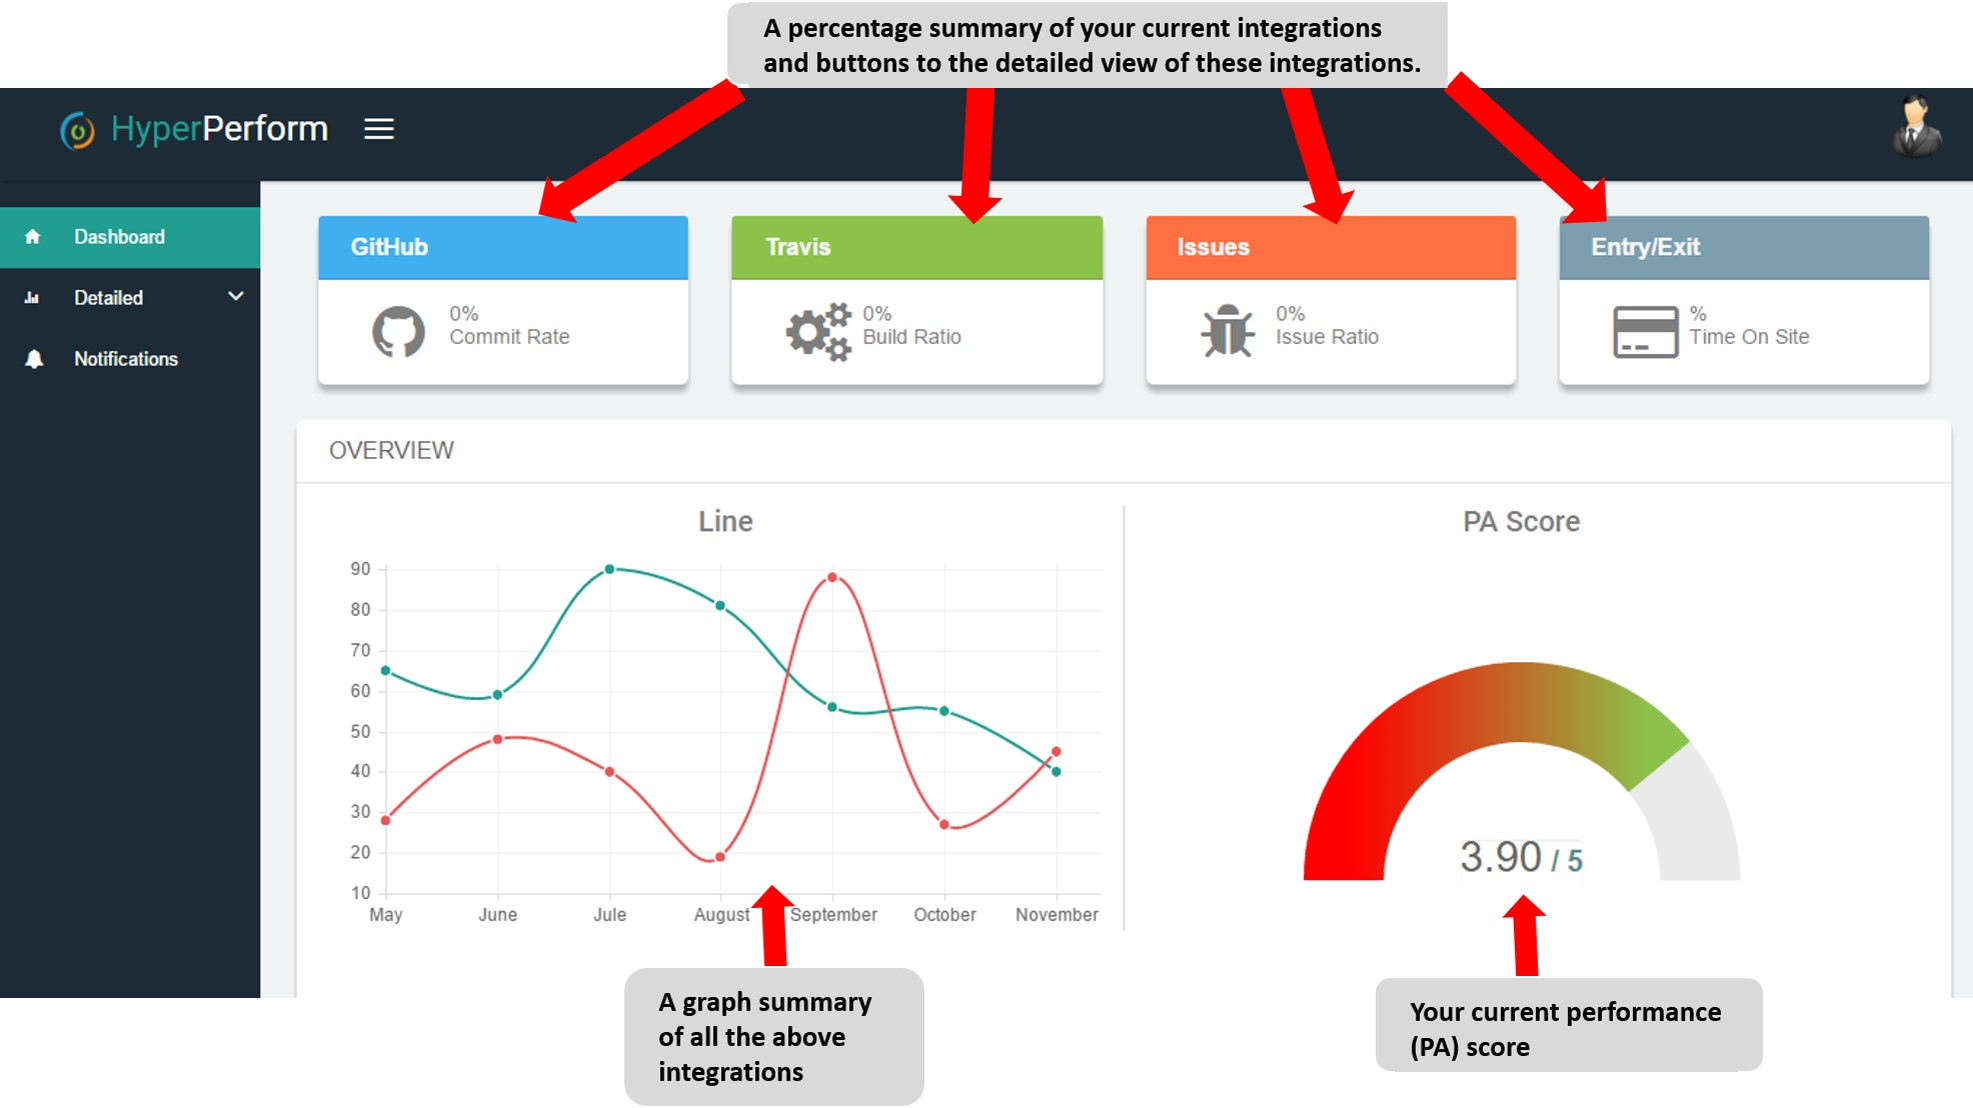
\includegraphics[scale=0.3]{../Images/dashboard.jpg}
		\caption{Dashboard}
	\end{center}
\end{figure}
\noindent
On this screen you are given a summarised view of all the integrations parts of the HyperPerform system. Note the four colour-coded panels on top, each of these panels represents an integration. These panels are click-able and will direct you to a details screen which will be discussed in the next section 5. \\ \\
If you wish to logout then you merely click on the profile icon in the top right corner. Once clicked you will be presented with a small menu. 

\begin{figure}[H]
	\begin{center}
		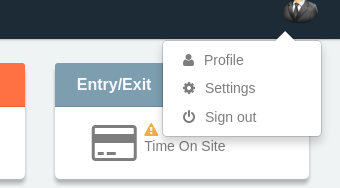
\includegraphics[scale=0.7]{../Images/logout}
		\caption{Dashboard}
	\end{center}
\end{figure}
\noindent
In this menu you have a few options to choose from. The Profile option will direct you to a profile page where you will be able to view and edit your current details. \\ \\
The second option is a simple settings page where you can customize the dashboard.\\ \\
And finally the Sign Out option can be used to log off the system. Once logged off you will be returned to the login screen in Figure 1.
\end{document}